\documentclass{beamer}
% Change theme
\usetheme{Antibes}
\usecolortheme{beaver}
% Change font
\usepackage[T1]{fontenc}
\usepackage[]{kpfonts}
% Use cleveref package
%\usepackage[capitalise]{cleveref}
% Use tikz
\usepackage[]{tikz}
\usetikzlibrary{backgrounds}
% Use bbm for blackboard things
\usepackage[]{bbm}
% AMS
\usepackage{amsmath}
\usepackage{hyperref}
%% Bibliography
%\usepackage[
%backend=biber,
%style=authoryear-comp,
%sorting=ynt,
%url=false,
%isbn=false,
%doi=false
%]{biblatex}
%\AtEveryBibitem{%
%  \clearfield{note}%
%  \clearfield{eprinttype}%
%  \clearfield{eprint}%
%}
%\addbibresource{Library.bib}
%% Pictures path
\graphicspath{{./pictures/}}
% Remove controls
\beamertemplatenavigationsymbolsempty 

% Title page information
\title{An Euler-Maruyama scheme for SDEs with distributional drift}
\author{Luis Mario Chaparro Jáquez}
\institute{University of Leeds\\School of Mathematics}
\date{October 14th 2022}
\logo{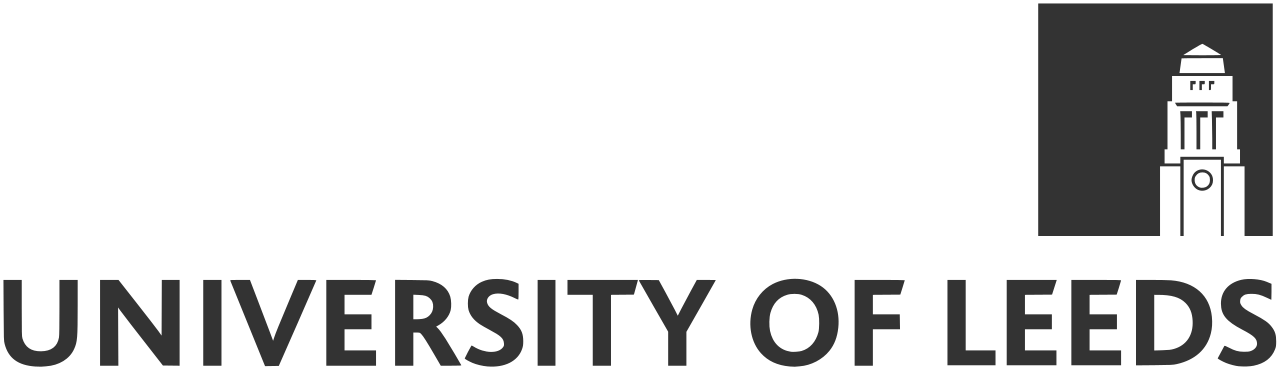
\includegraphics[width=25mm]{logo_leeds}}
% Table of contents at the beginning of each section
\AtBeginSection[]
{
  \begin{frame}{Table of Contents}
    \tableofcontents[currentsection]
  \end{frame}
}

\hypersetup{pdftitle={An Euler-Maruyama scheme for SDEs with distributional drift: Stats PGR Seminar 2022-23}, 
			pdfsubject={Probability, Numerical Analysis}, 
	        pdfauthor={Luis Mario Chaparro Jáquez},
			pdfkeywords={SDEs, Besov Space, Euler Scheme}
	       }

\begin{document}
\frame{\titlepage}
\frame{\tableofcontents}
\section{SDE with distributional drift}
\begin{frame}{The SDE}
	\begin{itemize}
	    \item
			Consider the SDE
			\begin{equation*}
				X_{t} = X_{0} + \int_{0}^{t} b(s, X_{s}) ds + W_{t},\,\,\,\,\,t \in [0, T]
			\end{equation*}
			where the drift
			$ b $
			belongs to the space of Schwartz distributions
			$ \mathcal{S}' $.
		\item
			In particular
			$ {\color{red}b \in C_T \mathcal{C}^{-\beta}(\mathbb{R})} := C([0, T];\mathcal{C}^{-\beta}(\mathbb{R})) $,
			%which is the space of continuous functions on time, taking values on the Zygmund-Hölder
			%$ \mathcal{C}^{-\beta} $
			for
			$ \beta \in (0, 1/4) $.
	\end{itemize}

	\begin{block}{Intuition}
	    Think of the coefficient
		$ -\beta $
		as the order of the existing ``derivatives'' of the functions in said space, or even better, the coefficient for a Hölder space.
	\end{block}
\end{frame}

\section{Euler-Maruyama scheme}
\subsection{Definition of the numerical scheme}
\begin{frame}{The numerical scheme}
	As in
	{\color{blue}De Angelis et al. 2022, Section 2.2},
	for an appropriate sequence
	$ b^{N} \to b $
	in
	$ C_T \mathcal{C}^{-\beta} $
	we can define an special Euler-Maruyama (E-M) scheme to approximate numerically the solution of the SDE for any
	$ t $
	\begin{equation*}
	    \label{eq:em_approx}
	    X^{Nm}_{t_{n+1}} 
		= 
	    X^{Nm}_{t_{n}} 
		+ 
		b^{N}\left(X^{Nm}_{t_{n}}\right) \Delta t_{n}
		+ 
		\Delta W_{t_{n}}
		.
	\end{equation*}
	%where
	%\begin{equation*}
	%    \label{eq:time_sup}
	%    k(t) = \sup \left\{ k: t_{k} \leq t \right\}.
	%\end{equation*}

	\begin{block}{Remark}
	    Note that a normal E-M scheme would only depend on 
		$ m $,
		whereas this scheme depends on
		$ h $
		and
		$ N $.
	\end{block}
\end{frame}

\subsection{Selection of the sequence $ b^{N} $}
\begin{frame}{What $ b^{N} $ to use}
	\begin{itemize}
		\item<1->
			Let
			$ p_{t} $
			be the heat semigroup.
		\item<2->
			We can define the approximated coefficient 
			$ b^{N} $
			by convoluting the heat kernel with the actual distributional coefficient. So that we have
			\begin{equation*}
			    \label{eq:conv_der}
			    b^{N}(x) := (p_{t(N)} \ast b)(x) = \int_{-\infty}^{\infty} p_{t(N)} (y) b(x - y) dy.
			\end{equation*}
	    \item<3->
			However, even though this integral is formally well posed by
			\textit{dual pairing}, 
			in practice we cannot compute it.
	\end{itemize}
\end{frame}

\begin{frame}{What $ b^{N} $ to use}
	\begin{itemize}
		\item<1->
			Let,
			$ B^{H}(x) $
			be
			\textbf{one path}
			of a fractional Brownian motion with Hurst parameter
			$ 0 < H < 1 $.

		\item<2->
			We can see that, 
			$ B^{H}(x) $
			is
			$ \alpha $-Hölder 
			continuous for any
			$ \alpha < H $
			and therefore its
			\textit{generalised derivative}
			belongs to
			$ \mathcal{C}^{\alpha-1} $
			({\color{blue}Issoglio 2013, Section 4.1}).

		\item<3->
			Therefore, we can select
			$ b := \frac{\partial}{\partial x} B^{H}(x) $,
			and since the derivative and convolution commute, the convolution of the previous slide is written as

			\begin{equation*}
			    \label{eq:conv}
			    b^{N}(x) := \left(p_{t(N)} \ast \frac{\partial}{\partial x} B^{H}\right)(x) = \left(\frac{\partial}{\partial x} p_{t(N)} \ast B^{H}\right)(x) 
			\end{equation*}
	\end{itemize}
\end{frame}

\section{Convergence rate}
\subsection{Some prior remarks}
\begin{frame}{Some remarks}
	\begin{itemize}
		\item<1-> 
			The convergence rate of an E-M scheme for an SDE with regular coefficients, i.e: Lipschitz continuous and with linear growth is known to be
		$ 1/2 $
		({\color{blue}Kloeden and Platen 1999, Section 10.2}).
		\item<2->
			However, 
		\textbf{our coefficients are not even functions!}
		\item<3->
			Moreover, since our E-M scheme depends on an additional parameter it is natural to expect a different rate, in particular one depending on the extra parameter.
	\end{itemize}
\end{frame}

\subsection{The convergence result}
\begin{frame}
	\begin{block}{Convergence rate of E-M scheme}
		Let
		$ X_{t} $
		be the solution to the SDE
		with drift coefficient
		$ b \in C_T \mathcal{C}^{-{\beta}} $,
		for
		$ {\beta} \in (0, 1/4) $
		and
		$ X^{Nm}_{t} $
		be the Euler approximation of the solution with
		$ m $
		time steps.
		Then it holds that
		\begin{equation*}
			\label{eq:euler_rate}
			\sup_{0 \leq t \leq T}
			\mathbb{E}
			\left[ \left| X^{Nm}_{t} - X_{t} \right| \right]
			\leq
			cm^{-\frac{1}{2} + \mu(\beta) + \epsilon},
		\end{equation*}
		where
		\begin{equation*}
			\label{eq:mu}
		  	\mu(\beta) = \frac{1}{2} \cdot \frac{{\beta}}{(1/2 - {\beta})(1 - 2 {\beta}) + {\beta}},
		\end{equation*}
		for any
		$ \epsilon > 0 $.
	\end{block}
\end{frame}

\begin{frame}{What does the previous result mean}
    \begin{itemize}
        \item<1->
			We care about the exponent of 
			$ m $, 
			which for the normal assumptions on the coefficients will be
			$ -1/2 $.
		\item<2->
			For
			$ {\beta} \to 0 $
			(measurable drift), we have an exponent
			\begin{equation*}
				-\frac{1}{2} + \underbrace{\frac{1}{2} \cdot 0}_{\lim_{\beta \to 0} \mu(\beta)} + \epsilon = \boxed{\color{red}-\frac12 + \epsilon}
			\end{equation*}
		\item<3->
			For
			$ {\beta} \to \frac14 $
			(distributional drift), we have an exponent
			\begin{equation*}
				-\frac12 + \underbrace{\frac{1}{2} \cdot \frac23}_{\lim_{\beta \to 1/4} \mu(\beta)} + \epsilon = \boxed{\color{red}-\frac16+ \epsilon}
			\end{equation*}
    \end{itemize}
\end{frame}

\begin{frame}[allowframebreaks]{References}
	\begin{itemize}
	    \item
			T. De Angelis, M. Germain, and E. Issoglio, ‘A numerical scheme for stochastic differential equations with distributional drift’, Stochastic Processes and their Applications, Sep. 2022, doi: 10.1016/j.spa.2022.09.003.
		\item
			E. Issoglio, ‘Transport Equations with Fractal Noise - Existence, Uniqueness and Regularity of the Solution’, Z. Anal. Anwend., vol. 32, no. 1, pp. 37–53, 2013, doi: 10.4171/ZAA/1473.
		\item
			P. E. Kloeden and E. Platen, Numerical solution of stochastic differential equations, Corr. 3rd print. Berlin; New York: Springer, 1999.
	\end{itemize}
\end{frame}
\end{document}
